\documentclass[matan]{subfiles}

\begin{document}
  \newpage
  \section{Применение интеграла Римана для вычисления площадей и объемов. Примеры.}

  \begin{definition} [школьное]
      Пусть $P \in \R^2$("фигрура"), $\mathcal{P}$ - некоторый набор плоских "фигур$"$, $P_i \in \mathcal{P}$

      $g: \mathcal{P} \rightarrow [0, +\infty)$ - называется площадью, если:
      \begin{enumerate}
          \item $\forall P \in \mathcal{P}$, $S(P) \geqslant 0$
          \item $\forall P_1, P_2 \in \mathcal{P}: P_1 \cap P_2 = \o$ $\Rightarrow$ $S(P_1 \cup P_2)=S(P_1)+S(P_2)$
          \begin{definition}
              $\uptau: \R^2 \rightarrow \R^2$, сохраняет расстояние
          \end{definition}
          \item $\forall P \in \mathcal{P}$ $\uptau$-движения $S(\uptau(P))=S(P)$
      \end{enumerate}
  \end{definition}

  \begin{center}
      \textbf{Площадь криволинейной трапеции.}
  \end{center}

  \begin{figure}[H]
      \centering
      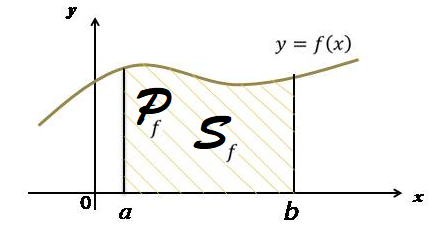
\includegraphics[width=6cm]{pics/31_1}
  \end{figure}

  \begin{definition}
      Подграфиком $f \in R[a,b]$ называется $P_f := \{(x,y)| a \leqslant x \leqslant b,\ 0 \leqslant y \leqslant f(x) \}$
  \end{definition}
  \\
  Возьмём разбиение и верх. и нижн. суммы Дарбу. $S$ - монотонна, т.е.

  $$P_1 \subset P_2 \Rightarrow S(P_1) \leqslant S(P_2),\ S_*(\uptau)=S(P_*(\uptau)),\ S^*(\uptau)=S(P^*(\uptau))$$

  $$P_*(f, \uptau) \subset P (f) \subset R^* (f, \uptau)$$
  \\
  \[\begin{matrix}
    S(P_*(f, \uptau)) = S_*(f, \uptau) \rightarrow \int_a^b f\\
    S(P^*(f, \uptau)) = S^*(f, \uptau) \rightarrow \int_a^b f
  \end{matrix}\qq \qq S(P_f) := \int_a^b f\]
  \newpage
  \begin{example}
      Первая четверть эллипса с радиусами $(a,b)$.

      \[\frac{x^2}{a^2} + \frac{y^2}{b^2} = 1,\q y = b \sqrt{1 - \frac{x^2}{a^2}},\q S = \int\limits_0^a b \sqrt{1 - \frac{x^2}{a^2}} dx\text{ - сложно, перейдём в поляры}\]
      $\begin{cases}
         x = a \cos t\\
         y = b \sin t
       \end{cases}$
       \[\int\limits_0^a f(x) dx = \int\limits_{\frac{\pi}{2}}^0 b \sin t d(a \cos t) = a b \int\limits_{\frac{\pi}{2}}^0 \sin^2 t dt = -a b (t - \frac{\sin 2t}{2}) |_{\frac{\pi}{2}}^0 = 0 - (-\frac{\pi a b}{4}) = \frac{\pi a b}{4}\]
  \end{example}

  \begin{center}
      \textbf{Вычисление объемов}
  \end{center}

  \begin{utv}
      Принцип Кавальери. Если у двух тел одни сечения на одном уровне, то их объемы равны.
  \end{utv}

  $\sum\limits_{k=0}^{n-1} S(\xi_k) \Delta_k$ - сумма Римана

  $V= \int\limits_a^b S(x) dx$ - измельчаем плоскости

  \begin{example}
      (на самом деле тела вращения можно считать как $V=\pi \int\limits_a^b f^2(x) dx$)
  \end{example}

  \newpage
  \section{Путь. Длина пути. Спрямляемый путь. Аддитивность длины пути.}

  \hypertarget{q32}{}

  \begin{definition}
      $\upgamma: [a,b] \rightarrow \R^n,\q \upgamma = \begin{pmatrix}
        \upgamma_ 1\\
        \upgamma_2\\
        ...\\
        \upgamma_n
      \end{pmatrix},\q \upgamma_k: [a,b] \rightarrow \R$.
      Расстояние считается как $d(x,y)=||x - y||_2=\sqrt{\sum\limits_{k=1}^n (x_k-y_k)^2}$, $\upgamma$ - путь, если $\forall i \in \{1,...k\}\ \upgamma_i \in C[a,b]$
  \end{definition}

  \begin{definition}
      Путь называется $r$-гладким, если $\forall i \in \{1,...k\}\ \upgamma_i \in C^r[a,b]$
  \end{definition}

  \begin{definition}
      Два пути считаются эквивалентными если можно сделать замену переменной. Т.е. пусть $\upgamma: [a,b] \rightarrow \R$, $\w{\upgamma}: [\upalpha, \upbeta] \rightarrow \R$, тогда:
      \\
      $\upgamma \sim \w{\upgamma}$ $\lra$ $\e \upvarphi: [a,b] \rightarrow [\upalpha, \upbeta]$ - строго возрастающая, $\upalpha = \upvarphi (a)$, $\upbeta = \upvarphi (b)$, $\upgamma = \w{\upgamma} \circ \upvarphi$
  \end{definition}

  \begin{definition}
      Кривая - класс эквивалентности путей. $\forall$путь - представитель класса эквивалентности называется "параметризацией"
  \end{definition}

  \begin{Example}
      \begin{equation*}
      \upgamma_1: \begin{cases}
         x = \cos t & 0 \leqslant t \leqslant 2 \pi\\
         y = \sin t & 0 \leqslant t \leqslant 2 \pi
      \end{cases}\ \ \ \ \ \ \ \ \ \ \ \
      \upgamma_2: \begin{cases}
         x = \cos t^2 & 0 \leqslant t \leqslant 2 \pi\\
         y = \sin t^2 & 0 \leqslant t \leqslant 2 \pi
       \end{cases}
      \end{equation*}
      $\upgamma_1 \sim \upgamma_2$, определяют одну и ту же кривую (окружность)
  \end{Example}

  \begin{definition}
      Кривая называется $r$-гладкой, если у неё есть $r$-гладкая параметризация
  \end{definition}

  \begin{definition}
      $\upgamma$ - простой путь $\lra$ $\upgamma$ - биекция на $(a,b)$, т.е. $\forall t_1, t_2 \in (a,b): \upgamma(t_1) \neq \upgamma(t_2)$ (без самопересечений). \\
  	Если $\upgamma(a) = \upgamma(b)$, $\upgamma$ - замкнутый путь.
  \end{definition}

  \begin{definition} [длины пути]
    	$\upgamma: [a,b] \rightarrow \R^m$, $\uptau - разбиение [a,b]: a=t_0<t_1<...<t_n=b$. Соединим $[\upgamma(t_k), \upgamma(t_{k+1})]$ отрезками - получим вписанную ломанную.
      $$\text{Длина $k$-ого звена: }\sqrt{\sum\limits_{j=0}^m (\upgamma_j(t_{k+1}) - \upgamma_j(t_k))^2}$$

      $$\text{Тогда длина вписанной ломанной: }l=\sum\limits_{k=0}^{n-1} \sqrt{\sum\limits_{j=0}^m (\upgamma_j(t_{k+1}) - \upgamma_j(t_k))^2}$$

      $$\text{Длиной пути назовём } S_\upgamma := \sup\limits_{\uptau} l_\uptau\text{ - всевозможных ломанных}$$
  \end{definition}

  \begin{definition}
      Путь называется спрямляемым, если $S_\upgamma < +\infty$
  \end{definition}

  \begin{utv}
      Аддитивность длины пути. $\upgamma: [a,b] \rightarrow \R$, $c \in (a,b)$, пусть $\upgamma_1$ - сужение $\upgamma$ на $[a,c]$, $\upgamma_2$ - сужение $\upgamma$ на $[c,b]$. Тогда $S_\upgamma = S_{\upgamma_1} + S_{\upgamma_2}$
  \end{utv}

  \begin{proof}
      а) $S_\upgamma \geqslant S_{\upgamma_1} + S_{\upgamma_2} ?$

      Пусть $\uptau_1$ - разбиение $[a,c]$, $\uptau_2$ - разбиение $[c,b]$,

      $\uptau = \uptau_1 + \uptau_2$, $l_{\uptau_1} + l_{\uptau_2} = l_\uptau \leqslant S_\upgamma$

      (т.к. $S_\upgamma - \sup$)

      Возьмём $\sup$ по всем разбиениям отрезка $[a,c]$

      $\Rightarrow$ $\sup\limits_{\uptau_1} (l_{\uptau_1} + l_{\uptau_2}) = S_{\upgamma_1} + l_{\uptau_2} \leqslant S_\upgamma$

      Теперь $\sup$ по всем разбиениям отрезка $[c,b]$

      $\Rightarrow$ $\sup\limits_{\uptau_1} (S_{\upgamma_1} + l_{\uptau_2}) = S_{\upgamma_1} + S_{\upgamma_2} \leqslant S_\upgamma$
      \\
      б) $S_\upgamma \leqslant S_{\upgamma_1} + S_{\upgamma_2} ?$

      Пусть $\uptau$ - разбиение $[a,b]$.

      Пусть $\uptau^* = \uptau \cup \{c\}$. $l_\uptau \leqslant l_{\uptau^*}$, $\uptau = \uptau_1 \cup \uptau_2$,

      где $\uptau_1$ - разбиение $[a,c]$, $\uptau_2$ - разбиение $[c,b]$.

      $l_\uptau \leqslant l_{\uptau^*} = l_{\uptau^1} + l_{\uptau^2} \leqslant S_{\upgamma_1} + S_{\upgamma_2}$

      Возьмём $\sup$ по всем разбиениям $\uptau$: $\sup\limits_{\uptau} (l_{\uptau}) = S_\upgamma \leqslant S_{\upgamma_1} + S_{\upgamma_2}$
  \end{proof}

  \begin{examples}
      Неспрямляемые пути:

      1) Кривая Пеано
      \begin{figure}[H]
          \centering
          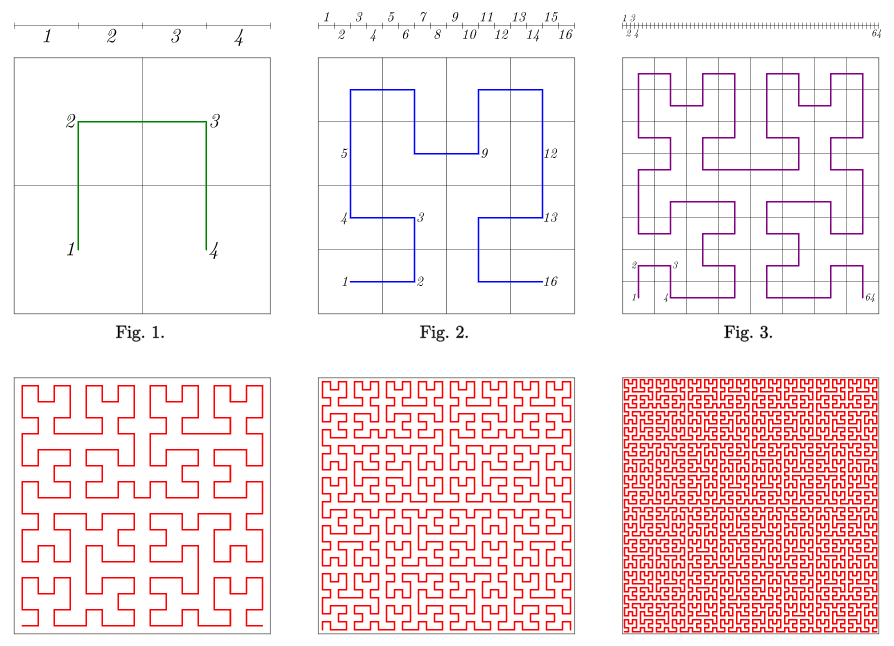
\includegraphics[width=9cm]{pics/32_1}
      \end{figure}

      В пределе $\upgamma: [0,1] \rightarrow [0,1]^2$ - сюръективное отображение. В итоге получается прямая заполняющая весь квадрат с пересеченями (в смысле дополнение до подкривых  пределе пусто)

      2) $y =
      \begin{cases}
         x \cos \frac{\pi}{x}, & x \neq 0\\
         0, & x = 0
       \end{cases}$

       \begin{figure}[H]
           \centering
           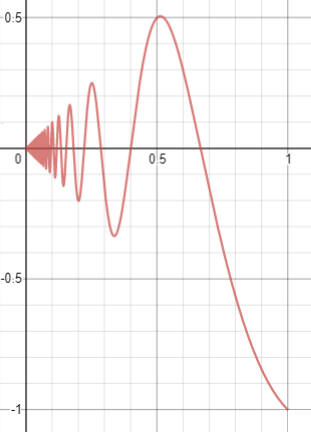
\includegraphics[width=3cm]{pics/32_2}
       \end{figure}

      Докажем, что прямая не является спямляемой.
      \\
      Пусть $\uptau: 0 < \frac{1}{N} < \frac{1}{N -1} < ... < 1$, $t_N = \frac{1}{N}$, тогда
      \[y(t_k) = \frac{1}{k} \cos \pi k = \frac{1}{k} (-\pi)^k\]
      Длина $k$-ого звена:
      \[\frac{1}{k} - (-\frac{1}{k+1}) \geqslant \frac{2}{k} \Rightarrow l_\uptau \geqslant \sum\limits_{k=1}^N  \frac{1}{k}\Rightarrow \sup l_\uptau = +\infty\]
  \end{examples}

  \newpage
  \section{Кривая. Длина кривой.}

  Опр. см. в билете \hyperlink{q32}{32}
  \begin{theorem} [о длинах эквивалентных путей]
      Пусть $\upgamma_1: [a_1,b_1] \rightarrow \R^m$, $\upgamma_2: [a_2,b_2] \rightarrow
      \R^m$. Если $\upgamma_1 \sim \upgamma_2$ $\Rightarrow$ $S_{\upgamma_1} = S_{\upgamma_2}$
  \end{theorem}

  \begin{proof}
      $\upgamma_1 \sim \upgamma_2$ $\Rightarrow$ $\e \upvarphi: [a_1, b_1] \rightarrow [a_2, b_2]$ - строго возрастающая, $\upgamma_1(t) = \upgamma_2(\upvarphi(t))$, $\upvarphi(\uptau_1) = \uptau_2$ - разбиение $[a_2,b_2]$,
      $$l_{\uptau_1} = \sum\limits_{k=0}^{n-1} \sqrt{\sum\limits_{j=0}^m (\upgamma_1(t_{k+1}) - \upgamma_1(t_k))^2} = l_{\uptau_2} \leqslant S_{\uptau_2}$$
      Перейдём к $\sup$ по всем $\uptau_1$: $\sup\limits_{\uptau_1} (l_{\uptau_1}) = S_{\uptau_1} \leqslant S_{\uptau_2}$

      Аналогично получим неравенство $S_{\uptau_2} \leqslant S_{\uptau_1}$
  \end{proof}

  \begin{remark}
      Корректность определения (с классами эквивалентности) длины пути следует из доказанной выше теоремы
  \end{remark}

  \newpage
  \section{Теорема о вычислении длины гладкого пути.}

  \begin{theorem}
      $\upgamma: [a,b] \rightarrow \R^m$ - $C^1$-гладкая кривая, тогда $\upgamma$ - спрямляется, $S_{\upgamma} = \int\limits_a^b |\upgamma'|$
  \end{theorem}

  \begin{proof}
      \\
      1) $\upgamma$ - спрямляемая?
      \\
      $\upgamma_j \in C^1[a,b]\ \forall j \in \{1,2,...,m\} \Rightarrow$(ф-ия достигает $\min$ и $\max$ на $[a,b]$ по т.Вейерштрасса)
      $$m_j \leqslant \upgamma_j \leqslant M_j,\ M := \sqrt{\sum\limits_{j=1}^m M_j},\ m := \sqrt{\sum\limits_{j=1}^m m_j},\ \upgamma' = \begin{pmatrix}
        \upgamma_1'\\
        \upgamma_2'\\
        ...\\
        \upgamma_n'
      \end{pmatrix}$$
      \\
      $\forall \uptau$-разбиения $[a,b]: l_\uptau = \sum\limits_{k=0}^{n-1} \sqrt{\sum\limits_{j=0}^m (\upgamma_1(t_{k+1}) - \upgamma_1(t_k))^2} = $
      \\
      (по т. Лагранжа $\forall k = 0,1,...n-1$ $\e \xi_k \in [t_k, t_{k+1}]: \upgamma_j(t_{k+1}) - \upgamma_j(t_k) = \upgamma_j'(\xi_k) \Delta_{t_k}$)
      \\
      $= \sum\limits_{k=0}^{n-1} \sqrt{\sum\limits_{j=0}^m (\upgamma_j'(\xi_k))^2 \Delta_{t_k}^2} = \sum\limits_{k=0}^{n-1} \sqrt{\sum\limits_{j=0}^m (\upgamma_j'(\xi_k))^2} \Delta_{t_k} \Rightarrow m \sum\limits_{k=0}^{n-1} \Delta_{t_k} \leqslant l_\uptau \leqslant M \sum\limits_{k=0}^{n-1}$
      \\
      $\Rightarrow m (b-a) \leqslant l_\uptau \leqslant M (b-a) \underset{sup}{\rightarrow} m (b-a) \leqslant S_\upgamma \leqslant M (b-a) \Rightarrow -\infty < S_\upgamma < +\infty$
      \\
      2) $S_{\upgamma} = \int\limits_a^b |\upgamma'|?$
      \\
      Пусть $\upgamma^{(k)}$ - сужение $\upgamma$ на $[t_k,t_{k+1}]$. Для него выполняется пункт (1):

      *переобозначим $\upgamma'$ как $\stackrel{\bullet}{\upgamma}$ из-за сложности обозначений*
      $$m_j^{(k)}=\min\limits_{t \in [t_k, t_{k+1}]} |\stackrel{\bullet}{\upgamma_j} (t)|,\ M_j^{(k)}=\max\limits_{t \in [t_k, t_{k+1}]} |\stackrel{\bullet}{\upgamma_j} (t)|$$
      $$m^{(k)} = \sqrt{\sum\limits_{j=1}^m (m_j^{(k)})^2},\ M^{(k)} = \sqrt{\sum\limits_{j=1}^m (M_j^{(k)})^2}$$
      $$m^{(k)} \Delta t_k \leqslant S_{\upgamma^{(k)}} \leqslant M^{(k)} \Delta t_k \Rightarrow \sum\limits_{k=1}^{n-1} \leqslant S_\upgamma \leqslant \sum\limits_{k=1}^{n-1} M^{(k)} \Delta t_k$$
      $$m_j^{(k)} \leqslant |\stackrel{\bullet}{\upgamma}_j^{(k)} (t) \leqslant M_j^{(k)}|\ t_k \leqslant t \leqslant t_{k+1},\ \forall j=1,...,m$$
      $$\text{Суммируем, возводим в квадрат, иззвлекаем корень:}$$
      $$m^{(k)} \leqslant |\stackrel{\bullet}{\upgamma}^{(k)} (t)| \leqslant M^{(k)}|\ t_k \leqslant t \leqslant t_{k+1}$$
      $$\text{Проинтегрируем по } \int\limits_{t_k}^{t_{k+1}} dt:\ m^{(k)} \Delta t_k \leqslant \int\limits_{t_k}^{t_{k+1}} |\stackrel{\bullet}{\upgamma}^{(k)} (t)| dt \leqslant M^{(k)} \Delta t_k$$
      $$\Rightarrow \sum\limits_{k=1}^{n-1} \leqslant \int\limits_{t_k}^{t_{k+1}} |\stackrel{\bullet}{\upgamma}^{(k)} (t)| dt \leqslant \sum\limits_{k=1}^{n-1} M^{(k)} \Delta t_k \text{, оценим } \sum\limits_{k=1}^{n-1} (M^{(k)} - m^{(k)} \Delta t_k):$$
      $$M^{(k)} - m^{(k)} = \frac{(M^{(k)})^2 - (m^{(k)})^2}{M^{(k)} + m^{(k)}} = \sum\limits_{j=1}^m (M_j^{(k)} - m_j^{(k)}) \frac{M_j^{(k)} + m_j^{(k)}}{M^{(k)} + m^{(k)}} \leqslant \sum\limits_{j=1}^m (M_j^{(k)} - m_j^{(k)})$$
      $$\upgamma_j \in C^1 [a,b] \Rightarrow \upgamma_j' \in C[a,b] \Rightarrow \text{р/н} \lra \forall \E > 0\ \e \updelta_j > 0:$$
      $$\uplambda(\uptau) < \updelta_j \Rightarrow 0 \leqslant M_j^{(k)} - m_j^{(k)} \leqslant \frac{\E}{m(b-a)} \underset{\updelta = \underset{1 \leqslant j \leqslant m}{\min \updelta_j}}{\stackrel{\sum\limits^m}{\Rightarrow}} 0 \leqslant M^{(k)} - m^{(k)} \leqslant \frac{\E}{b-a}$$
      $$\Rightarrow \sum\limits_{k=0}^{n-1} (M^{(k) - m^{(k)}} \Delta t_k < \frac{\E}{b-a} \sum\limits_{k=0}^{n-1} \Delta t_k = \E \Rightarrow S_\upgamma = \int\limits_a^b |\stackrel{\bullet}{\upgamma}|$$
  \end{proof}

  \newpage
  \section{Функциональные последовательности и ряды. Поточечная и равномерная сходимость. Примеры.}

  \begin{Definition}
      \[f_n : E \to \R \q E \subset \R\]
  	\[\text{Говорят, что функ. последовательность сходится поточечно к $f : E \to \R$, если:}\]
  	\[\forall x \in E \q \forall \mathcal{E} > 0 \q \exists N_{(x, \mathcal{E})} : \q \forall n > N \q \abs{f_n(x) - f(x)} < \mathcal{E}\]
  \end{Definition}

  \begin{Definition}
      \[\text{Говорят, что функ. послед. сходится к f равномерно на } E\]
  	\[f_n \us{E}{\rightrightarrows} f \]
  	\[\text{Если } \sup_{x \in  E} \abs{f_n(x) - f(x)} \us{n \to \infty}{\to 0}\]
  	\[\rla \forall \mathcal{E} > 0 \q \exists N_{(\mathcal{E})} \q \forall n > N \q \sup_{x \in E} \abs{f_n(x) - f(x)} < \mathcal{E}\]
  	\[\rla \forall \mathcal{E} > 0 \q \exists N_{(\mathcal{E})} \q \forall n > N \q \forall x \in E \q \abs{f_n(x) - f(x)} < \mathcal{E} \]
    \begin{figure}[H]
        \centering
        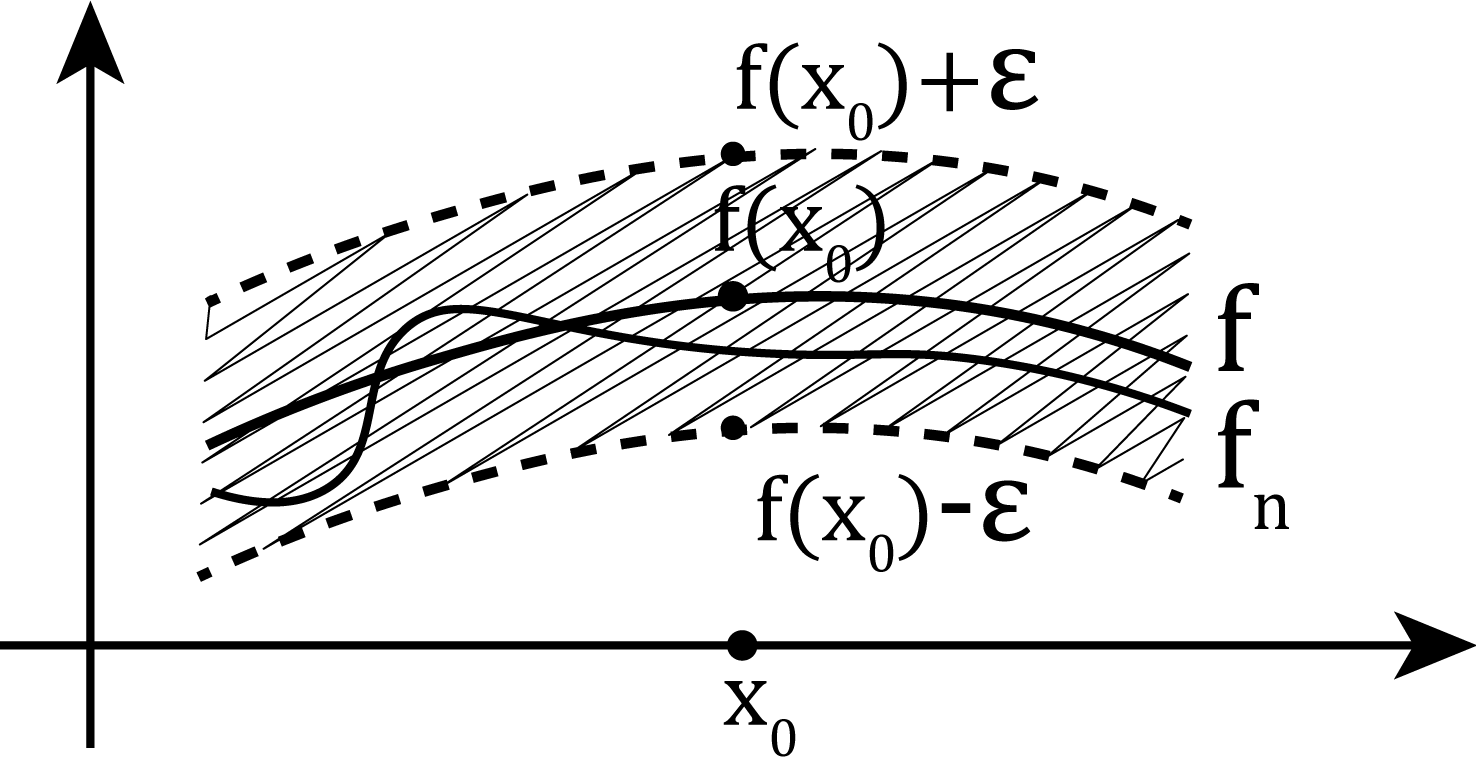
\includegraphics[width=6cm]{pics/35_1.png}
    \end{figure}
  \end{Definition}

  \begin{examples}
  		\begin{enumerate}
  			\item $\displaystyle  f_n(x) = \frac{sin^2(e^x) - \arctan(n^2 \sqrt{x})}{\sqrt{n}} \q\q x \in [0; +\infty)$
  				\[0 \leq \sup_{[0, +\infty)} \abs{f_n(x)} \leq \frac{10}{\sqrt{n}} \to 0 \]
  				\[\Ra f_n \us{[0, + \infty)}{\rightrightarrows} 0\]
  			\item $f_n(x) = x^n - x^{2n} \q\q x \in [0, 1] $
  				\[f_n(x) \us{n \to \infty}{\to } 0 \q \forall x \in [0, 1] \text{ - поточечно. Равномерно ли?}\]
  				\[f'_n(x) = n x ^{n - 1} - 2nx^{2n-1} = x^{n - 1}(n - 2nx^n)\]
  				\[x_n = \frac{1}{\sqrt[n]{2}} \text{ - крит. точка}\]
  				\[f_n(x_n) = \frac{1}{2} - \frac{1}{4} = \frac{1}{4}\]
  				\[\Ra \sup_{x \in [0, 1]} \abs{f_n(x)} = \frac{1}{4} \Ra \text{ равномерной сх-ти нет}\]
          \begin{figure}[H]
              \centering
      		    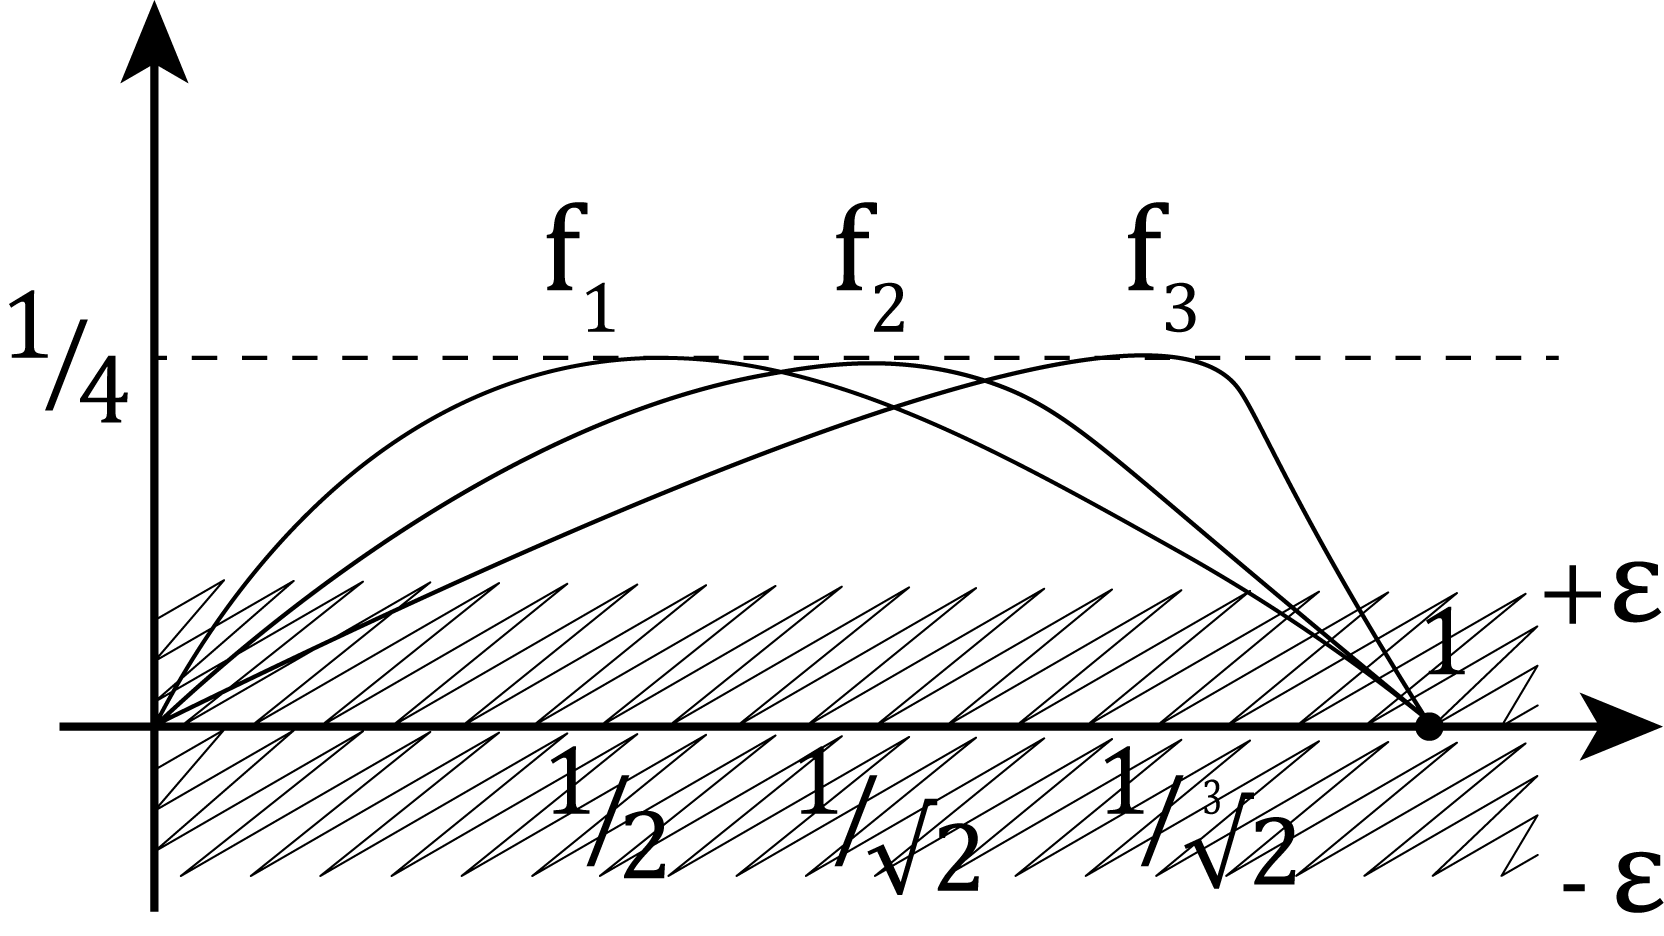
\includegraphics[width=6cm]{pics/35_2.png}
              \caption{Горбик убегает}
      		\end{figure}
  		\end{enumerate}
  \end{examples}

  \begin{remark}
  		Из равномерной сх-ти $\Ra$ поточечная
  \end{remark}

  \newpage
  \section{Критерий Коши для равномерной сходимости функциональной последовательности.}

  \begin{Theorem} [Критерий Коши для равномерной сходимости функ. послед.]
  		\[f_n \us{E}{\rightrightarrows} f \rla \forall \mathcal{E} > 0 \q \exists N_\mathcal{E} :
  		\forall m, n > N_\mathcal{E} \q\q \sup_{x \in E} \abs{f_n(x) - f_m(x)} < \mathcal{E} \]
  \end{Theorem}

  \begin{proof}
    ($\Ra$):
  	\[f_n \rightrightarrows f \rla \sup \abs{f_n(x) - f(x)} \to 0\]
    \[\Ra \forall \mathcal{E} > 0 \q \exists N_\mathcal{E} > 0: \q \forall m, n > N_\mathcal{E} :\]
    \[\qq \sup \abs{f_n - f_m} \leq
        \sup(\abs{f_n - f} + \abs{f - f_m})
        < \frac{\mathcal{E}}{2} + \frac{\mathcal{E}}{2} = \mathcal{E}\]
    ($\La$):
  	\[\forall x \in E \q \forall \mathcal{E} > 0 \q \exists N_\mathcal{E} :
  	\forall m, n > N_{\mathcal{E}} \q \abs{f_n(x) - f_m(x)} < \mathcal{E}\]
  	\[\text{т.е. } \{f_n(x)\} \text{ - сх. в себе } \rla \{f_n(x)\} \text{ имеет конеч. предел}\]
  	\[f(x) = \lim_{n \to \infty} f_n(x),  \text{ т.о. } f_n(x) \to f(x) \q \forall x \in E\]
    \[\qq \text{(т.е. f - поточеч. предел послед.)}\]
  	\[\forall \mathcal{E} > 0 \q \exists N_\mathcal{E} : \forall m, n > N_\mathcal{E} \q \forall x \in E\]
  	\[f_m(x) - \mathcal{E} < f_n(x) < f_m(x) + \mathcal{E} \us{n \to \infty}{\ra}
  	  f_m(x) - \mathcal{E} \leq f(x) \leq f_m(x) + \mathcal{E}\]
  	\[\Ra \abs{f_m(x) - f(x)} \leq \mathcal{E} < 2 \mathcal{E}\]
  	\[\Ra \sup \abs{f_m(x) - f(x)} < \mathcal{E}\]
  \end{proof}

  \newpage
  \section{Сохранение непрерывности при равномерном предельном переходе. Теорема Дини (б/д). Теорема о предельном переходе под знаком интеграла.}

  \begin{Theorem} [о равномерном пределе непр. функции]
  		\[f_n \text{ - непр в т. } x_0 \in E, \qq f_n \us{E}{\rightrightarrows} f\]
  		\[\text{Тогда } f \text{ - непр. в т. } x_0\]
  \end{Theorem}

  \begin{Proof}
  	\[\forall \mathcal{E} > 0 \q(\text{зафиксир.), т.к. } f_n \rightrightarrows f \text{, то:}\]
    \[\exists N_\mathcal{E} : \forall n > N_\mathcal{E} \q (\text{зафикс } n^* > N_\mathcal{E}) \q \sup_E \abs{f_n - f} < \frac{\mathcal{E}}{3}\q (*)\]
  	\[\text{В частности, для } n^* > N_\mathcal{E} \q \sup_E \abs{f_{n} - f} < \frac{\mathcal{E}}{3}\]
  	\[\qq f_{n^*} \text{ - непр. в т. } x_0 : \q \exists \delta > 0 \q \forall t \in E : \q
  	\abs{t - x_0} < \delta \q \abs{f_{n^*}(t) - f_{n^*}(x_0)} < \frac{\mathcal{E}}{3}\]
  	\[\text{Тогда } \forall x \in E : \q \abs{x - x_0} < \delta\]
  	\[ \qq \abs{f(x) - f(x_0)} \os{\bigtriangleup
  }{\leq} \abs{f(x) - f_{n^*}(x)} + \abs{f_{n^*}(x) - f_{n^*}(x_0)} + \abs{f_{n^*}(x_0) - f(x_0)} < \mathcal{E}\]
  \end{Proof}

  \begin{Consequence}
  	\[\text{Если } f_n \in C(E), \q f_n \us{E}{\rightrightarrows} f \text{, то } f \in C(E)\]
  \end{Consequence}

  \begin{Theorem} [Дини]
  	\[f_n \in C[a, b] \q\q f_n(x) \to f(x) \q(\text{поточ. на $[a, b]$})\]
  	\[\text{Причем}\q \forall x \in [a, b] \q f_n(x) \searrow \text{ (по n) } (f_n \searrow f), \text{ т.е } f_{n+1}(x) \leq f_n(x) \]
  	\[\text{Если } f \in C[a, b] \text{, то } f_n \us{[a, b]}{\rightrightarrows} f\]
  \end{Theorem}

  \begin{Proof}[не нужно доказывать]
    \[\text{Т.к. } f_n \searrow f, \text{ то}\q \forall x \in [a,b] \q \forall \E > 0 \q \e N_{\E,x}: \forall n > N_{\E,x} \q 0 \leq f_n(x) - f(x) < \E\]
    \[n_x \text{ - зафикс. } (n_x > N_{\E,x})\]
    \[f_{n_x}-f \text{ - непр. на $[a,b]$ и в т. x}\]
    \[\Ra \e U_x \text{-окр.: } \forall t \in U_x \q 0 \leq  f_{n_x}(t)-f(t) < \E \q (*)\]
    \[\text{и по т. о стабилизации знака в каждой x выбираем окр. такую что:}\]
    \[[a,b] \subset \us{x \in [a,b]}{\cap} U_x \Ra \e \{x_j\}_{j=1}^N: [a,b] \subset \os{N}{\us{j=1}{\cap}} U_{x_j} \]
    \[\text{(компакт, значит можем выделить конечное подпокрытие)}\]
    \[n_{\E} := \max_{1 \leq j \leq N}(n_{x_j}) \text{ - номера $f_n$ для $\forall x_j$ такие что $(*)$:}\]
    \[\forall \xi \in [a,b] \q \e j = 1...N: \xi \in U_{x_j} \Ra \forall n> n_{\E} > n_{x_j}\]
    \[0 \leq f_n(\xi) - f(\xi) < \E\]
  \end{Proof}

  \begin{Theorem} [о предельном переходе под знаком интеграла]
  	\[f_n \in R[a, b] \q f_n \us{[a, b]}{\rightrightarrows} f \in R[a, b]\]
  	\[\text{Тогда } \int_a^b f_n \us{n \to \infty}{\to } \int_a^b f\]
  \end{Theorem}

  \begin{Proof}
  		\[a < b\]
  		\[\abs{\int_a^b f_n - \int_a^b f} \leq \int_a^b \abs{f_n - f} <
  			\sup_{[a, b]} \abs{\us{\to 0}{f_n - f}} \cdot (b-a) \to 0\]
  \end{Proof}

  \begin{utv}
  		Функ. ряд сход равномерно $\rla$ посл-ть частичных сумм сход равномерно
  \end{utv}

  \begin{Consequence}[1]
  	\[f_n \in C[a, b] \q \sum_{n = 1}^N f_n \rightrightarrows f, \text{ тогда:}\]
  	\[\begin{align}
  		&\q1) \q f(x) = \sum_{n = 1}^\infty f_n \in C[a, b] \\
  		&\q2) \q \int \sum_{n = 1}^\infty f_n = \sum_{n = 1}^\infty \int f_n
  	\end{align}\]
  \end{Consequence}

  \begin{Consequence}[2]
  	\[\text{Если } f_n(x) \geq 0 \q \forall  x \in [a, b] \q\q f_n \in C[a, b]\]
  	\[\sum_{n = 1}^\infty f_n = f \in C[a, b] \]
  	\[\text{То } \sum f_n \text{ - сход. равномерно на } [a, b]\]
  \end{Consequence}
  \newpage
  \section{Дифференцируемость и равномерная сходимость.}

  \begin{Theorem} [диф-сть и равном. сх-ть]
  	\[f_n \in C^{1}[a, b] \q f_n' \us{[a, b]}{\rightrightarrows} g\]
  	\[\text{и } \exists c \in [a,b] : \q \{f_n(c)\}^\infty_{n = 1} \text{ - сх} \]
  	Тогда:
    \begin{enumerate}
      \item $f_n \rightrightarrows f \text{ на } [a, b]$
      \item $f \in  C^1[a, b] \text{ и } f' = g$
    \end{enumerate}
  \end{Theorem}

  \begin{Proof}
    \[1. \q \text{Покажем, что } f_n \rightrightarrows f\]
  	\[\sup_{x \in [a, b]} \abs{f_n(x) - f(x)} = \sup \abs{\textcolor{red}{f_n(x) - f_n(c)} + f_n(c) - f(c) + \textcolor{blue}{f(c) - f(x)}} \leq \]
  	\[\leq \sup \abs{\textcolor{red}{\int_c^x f'_n} - \textcolor{blue}{\int_c^x g} + f_n(c) - f(c)} \leq
  	\sup \abs{\int_c^x (f'_n - g)} + \abs{f_n(c) - f(c)} \q (*)\]
  	\[f'_n \rightrightarrows g \Ra \abs{\int_c^x (f'_n - g)} \leq \underbracket{\sup \abs{ f'_n - g}}_{\to 0}
  	\underbracket{(x-c)}_{\leq (a - b)} \]
  	\[\forall  \mathcal{E} > 0 \q \exists N : \forall n > N \q \abs{\int_c^x (f_n' - g)} < \mathcal{E}\]
  	\[\exists N_2 : \forall n > N_2 \q \abs{f_n(c) - f(c)} < \mathcal{E} \Ra (*) < 2\mathcal{E} \Ra f_n \rightrightarrows f\]
  	\begin{multline*}
  		2. \q f_n(x) - f_n(c) = \int_c^x f'_n \us{n \to \infty}{\to } \int_c^x g \os{1.}{\us{(*)}{=}} f(x) - f(c) \ \os{1.}{\Ra} \
  		f(c) = \lim_{n \to \infty} f_n (c) \\
  		\text{ (по т. о 		предельном переходе под знаком интеграла)}
  	\end{multline*}
  	\[\os{(*)}{\Ra} f(x) = \int_c^x g + f(c) \Ra f'(x) = g\]
  	\[\text{т.о}\q f_n(x) \to f(x) \text{ поточ. на }[a, b]\]
    \[f'(x) = g(x) \text{ непр. (равн. предел непр ф.)}\]
  	\[\Ra f \in C^1[a, b]\]
  \end{Proof}

  \begin{Example}
  	\[f_n(x) = \frac{1}{n} \arctan(x^n)\]
  	\[\sup_{\R} \abs{f_n(x)} \leq \frac{\pi}{2n} \to 0 \q \text{ т.е. } f_n \us{\R}{\rightrightarrows} 0 = f\]
  	\[f'_n(1) = \frac{1}{n} \cdot \frac{1}{1 + x^{2n} } \cdot n \cdot x^{n - 1} \bigg|_1 = \frac{1}{2}\]
  	\[\text{Но } (\lim_{n \to \infty}  f_n)'_{x = 1} = 0 \neq \lim_{n \to \infty} f_n'(1) \]
  \end{Example}

  \newpage
  \section{Признак Вейерштрасса равномерной сходимости функциональных рядов.}

  \begin{Theorem} [признак Вейерштрасса равн сх-ти]
  		\[f_n : E \to \R\]
  		\[\forall n \ \exists M_n: \q \abs{f_n(x)} \leq M_n \q \forall x \in E\]
  		\[\sum_{n = 1}^\infty M_n < \infty \text{ (сход. мажоранта)} \]
  		\[\text{Тогда ряд } \sum_{n = 1}^\infty f_n(x) \text{ сх. равномерно и абсолютно на } E\]
  \end{Theorem}

  \begin{Proof}
  	\[\sum_{n = 1}^\infty M_n < \infty \Ra \forall \mathcal{E} > 0 \q \exists N: \forall m, n > N
  	\rla \sum M_k < \infty\]
  	\[\text{Тогда } \abs{S_n - S_{m - 1}} = \abs{\sum_{k = m}^n f_k(x)} \leq \sum_{k = m}^n \abs{f_k(x)} \leq
  	\abs{\sum_{k = m}^n M_k } < \mathcal{E}\]
  	\[\text{Т.е. } \abs{S_n - S_{m - 1} } < \mathcal{E}, \text{ т.е. вып. кр. Коши для } S_n(x) =
  	\sum_{k = 1}^n f_k(x) \]
  	\[\text{част. суммы сх равн. } \Ra \text{ функ. ряд сх. равн.}\]
  \end{Proof}

  \begin{TTheorem}[Вейерштрасса о плотности алгебраических многочленов в C[a,b{]}]
  \[\text{Пусть } f \in C[a,b], \text{ тогда} \q \forall \E > 0 \q \e P(x): \max_{x \in [a,b]} |f(x) - P_n(x)| < \E\]
  \end{TTheorem}

  \begin{LLemma}
    \[\begin{enumerate}
      \item \sum_{k=0}^n C_n^k x^k (1-x)^{n-k} = (x+1-x)^n = 1^n
      \item \sum_{k=0}^n C_n^k (\frac{k}{n} - x)^2 x^k (1-x)^{n-k} = \frac{x(1-x)}{n}
    \end{enumerate}\]
  \end{LLemma}

  \begin{DDefinition}
    \[b_{k,n}(x) = C_n^k x^{k} (1-x)^{n-k}, \qquad k=0,\ldots,n\]
    \[B_n(f; x) = B_n(x) = \sum_{k=0}^{n} f\left(\frac{k}{n}\right) b_{k,n}(x) \text{ - многочлен Бернштейна}\]
  \end{DDefinition}
  \[\sup|f(x)-B_n(x)| < \E\]

  \newpage
  \section{Степенной ряд (в $\CC$). Радиус сходимости. Формула Коши-Адамара.}

  \begin{Definition}
      \[\text{Будем рассматривать }\]
  	\[\sum_{k = 0}^\infty c_k z^k \q\q c_k, z \in  \CC \]
  \end{Definition}

  \begin{Definition}
    \[z = x + iy\]
  	\[x = \real z \qq y = \im z\]
  	\[\abs{z} = \sqrt{x^2 + y^2}\]
  	\[x = \abs{z} \cos{\varphi} \qq y = \abs{z} \sin{\varphi}\]
  	\[\abs{z_1 - z_2} = \sqrt{(x_1 - x_2)^2 + (y_1 - y_2)^2}\]
  	\[C_n = a_n + i b_n \q n \in \N\]
  	\[\lim_{n \to \infty} c_n = c \text{, если } \forall \mathcal{E} > 0 \q \exists N : \forall n > N
      \q \abs{c_n - c} < \mathcal{E}\]
  \end{Definition}

  \begin{utv}
    Пусть $c_n = a_n + i b_n,\text{ где\q} a_n, b_n \in \R,$
    \[c = a + ib\qq a,\text{ где\q} b \in \R,\text{ тогда:}\]
		\[c_n \us{n \to \infty}{\to } c \rla \begin{align}
			&a_n \to a\\
			&b_n \to b
		\end{align} \q (n \to \infty)\]
  \end{utv}

  \begin{proof}
    $(\Ra)$:
    \[|c_n - c| \ra 0\ \Ra\ \max(|a_n - a|,\ |b_n - b|) \ra 0\ \Ra\ a_n \ra 0 \q b_n \ra b\]\\
    $(\La)$:
    \[\max(|a_n - a|,\ |b_n - b|) \leq |c_n - c| = \sqrt{(a - a_n)^2 + (b - b_n)^2}\]
    (максимум из катетов не превосходит гипотенузу)
  \end{proof}

  \begin{Lemma}
    \[\text{Если }z^* \neq 0 \in \CC,\q \sum c_k |z^*| < \infty\]
    \[\text{Тогда } \forall d < 1 \q \sum c_k z^k \text{ - сх. равн. в круге } |z| \leq d |z^*|\]
  \end{Lemma}

  \begin{remark}
    Признак Вейерштрасса работает и в $\CC$
  \end{remark}

  \begin{Proof}
    \[|c_n z^n| \leq |c_n {z^*}^n|\abs{\frac{z}{z^*}}^n \os{|z| \leq d |z^*|}{\leq} \us{\ra 0 \Ra \text{огр.}}{|c_n {z^*}^n}|} d^n \leq \const d^n\]
    \[\Ra \text{ по пр. Вейерштрасса } \sum c_n z^n \text{ - сх. равн. и абс.}\]
  \end{Proof}

  \begin{consequence}
    Если $z_0: \sum c_n z_0^n $ - расх. $\Ra \forall z: |z| > |z_0| \sum c_n z^n$ расх.
  \end{consequence}

  \begin{definition}
  	Радиусом сх-ти степ. ряда $\sum c_n z^n$ назыв $R \in [0, +\infty]$ такое, что $(z \neq 0)$
  	\[\forall z : \abs{z} < R \text{ - ряд. сх}\]
  	\[\forall z : \abs{z} > R \text{ - ряд расх.}\]
  \end{definition}

  \begin{examples}

  		\begin{enumerate}
  			\item $\displaystyle \sum_{k = 0}^\infty k! z^k \text{ по пр. Даламб \q расх }
  				\forall z \neq 0 \q R = 0$
  				\[\lim_{k \to +\infty} \frac{\abs{(k + 1)! z^{k + 1}}}{\abs{k!z^k}} = \infty, \q z \neq 0\]
  			\item $\displaystyle \sum_{k = 0}^\infty \frac{z^k}{k!} \text{ - сх. } \forall z \in \CC$
  			\item $\displaystyle \sum_{n = 1}^\infty \frac{z^n}{n} \q\q $
  				\[\begin{align}
  					&z^* = -1& : \q &\sum \frac{(-1)^n}{n} \text{ - сх } \Ra \text{ сх. равн. }
  					\forall \abs{z} \leq d < 1\\
  					&z_0 = 1& : \q &\sum \frac{1}{n} \text{ - расх } \Ra \forall \abs{z} > 1
  				\end{align}\]
  		\end{enumerate}
  \end{examples}

  \begin{Theorem} [ф-ма Коши-Адамара]
  		\[\sum_{k = 0}^\infty c_k z^k \q R \text{ - рад. сх-ти} \]
  		\[\frac{1}{R} = \overline{\lim_{k \to \infty} } \sqrt[k]{\abs{c_k}}\]
  \end{Theorem}

  \begin{proof}
    *здесь когда-нибудь будет док-во*
  \end{proof}

  \begin{Upr}[1]
    \[\sum a_k z^k \text{ - ряд сх. в $R_a$}\]
    \[\sum b_k z^k \text{ - ряд сх. в $R_b$}\]
    \[\sum c_k z^k \text{ - ряд сх. в $R_c$}\]
    \begin{enumerate}
      \item Д-ть, что $R_c \geq \min(R_a, R_b)$
      \item Бывает ли >?
      \item =?
    \end{enumerate}
  \end{Upr}

  \begin{Upr}[2]
    \[\sum_{k=0}^{\infty} c_k z^k \text{ - радиус сх-ти $R$}\]
    Доказать, что у $\sum\limits_{k=1}^{\infty} c_k k z^{k-1}$ радиус сх-ти такой же
  \end{Upr}
\end{document}
